\documentclass[letterpaper,journal]{IEEEtran}
% chktex-file 1
% chktex-file 2
% chktex-file 3
% chktex-file 8
% chktex-file 12
% chktex-file 13
% chktex-file 18
% chktex-file 24
% chktex-file 35
% chktex-file 44
\usepackage{amsmath,amsfonts}
\usepackage{algorithmic}
\usepackage{algorithm}
\usepackage{array}
\usepackage[caption=false,font=normalsize,labelfont=sf,textfont=sf]{subfig}
\usepackage{textcomp}
\usepackage{stfloats}
\usepackage{placeins}
\usepackage{url}
\usepackage{verbatim}
\usepackage{adjustbox}
\usepackage{graphicx}
\usepackage{cite}
\IfFileExists{ConferencePaperNAPS_MLL/img/brazil_sys.png}{%
	\graphicspath{{ConferencePaperNAPS_MLL/img/}}%
}{%
	\graphicspath{{img/}}%
}
\hyphenation{op-tical net-works semi-conduc-tor IEEE-Xplore}
\raggedbottom
% updated with editorial comments 8/9/2021

\begin{document}

% \title{A Sample Article Using IEEEtran.cls\\ for IEEE Journals and Transactions}
\title{{\fontsize{24pt}{24pt}\selectfont An Open-source and Optimization-based\\ AC/DC Power Flow Model for the Brazilian Interconnected Power System}}

% \author{
%     Marck Llerena-Velasquez, Fernando Liederer, Marcos J. Rider, Daniel Dotta\\
%     {\small \textit{Department of Electrical and Computer Engineering}}\\
%     {\small \textit{State University of Campinas}}\\
%     {\small \textit{Campinas, SP, Brazil}}
% }

% \author{
% \IEEEauthorblockN{Marck Llerena-Velasquez\IEEEauthorrefmark{2}, Marcos J. Rider\IEEEauthorrefmark{2} and Daniel Dotta\IEEEauthorrefmark{2}}\\
% \IEEEauthorblockA{\textit{\IEEEauthorrefmark{2}State University of Campinas (UNICAMP)}\\
% Campinas, Brazil\\marck.llerena-velasquez@nlr.gov, dottad@unicamp.br }
% }

\author{
	\IEEEauthorblockN{Marck Llerena Velasquez\IEEEauthorrefmark{2}, Marcos J. Rider\IEEEauthorrefmark{2} and Daniel Dotta\IEEEauthorrefmark{2}}\\
	% \vspace{0.1cm}
	\IEEEauthorblockA{\IEEEauthorrefmark{2}\textit{State University of Campinas (UNICAMP), Campinas, Brazil}} \\
	% \IEEEauthorblockA{\IEEEauthorrefmark{3}\textit{National Laboratory of the Rockies, Colorado, USA}} \\
	\IEEEauthorblockA{marck.llerena-velasquez@nlr.gov, dottad@unicamp.br}
}
% The paper headers
\markboth{}%
{Shell \MakeLowercase{\textit{et al.}}: An Open-source and Optimization-based AC/DC Power Flow Model for the Brazilian Interconnected Power System}

\IEEEpubid{}
% Remember, if you use this you must call \IEEEpubidadjcol in the second
% column for its text to clear the IEEEpubid mark.

\maketitle

\begingroup
\hbadness=10000
\begin{abstract}
	This paper introduces an open-source optimization-based integrated AC/DC power flow model for complex hybrid grids such as the Brazilian Interconnected Power System (BIPS). The nonlinear programming (NLP) formulation combines AC balance, detailed steady-state line-commutated converter (LCC), and FACTS equations. Signed residual variables, bounded both per bus and in aggregate, provide a measurable feasibility criterion while weighted regularization keeps the solution near the scheduled operating state. The model was implemented in Python/Pyomo, solved with Ipopt, and validated against Anarede on an equivalent BIPS case. Scalability tests converged for all six cases, including three 11,250-bus snapshots in 21.3--23.2~s total time. In direct load-stress tests, the NLP solved five of nine scenarios, compared with three of nine for Newton-based entries, although all solved benchmark points retained voltage or branch-limit violations. The results therefore support improved numerical robustness and large-system tractability, while separating power-balance convergence from operational acceptability.

\end{abstract}
\endgroup

\begin{IEEEkeywords}
	FACTS, hybrid AC/DC systems, large-scale power systems, LCC-HVDC, nonlinear programming, open-source software, static var compensator, thyristor-controlled series capacitor.
\end{IEEEkeywords}

\section{Introduction}


Power flow analysis is a fundamental process in power systems operations and planning, since it provides the steady-state voltages, 
angles, and power injections used in security assessment and grid studies \cite{ref1}. For many years, this process has been solved mainly 
with Newton Raphson and Fast Decoupled methods, which offer good computational performance for conventional AC networks. As modern grids evolve, 
however, the modeling scope has expanded beyond the traditional AC setting. The growing integration of FACTS devices and HVDC systems introduces 
high nonlinearities, which increases the complexity of the power flow problem \cite{ref2}.
In hybrid AC/DC systems, representations are separated into sequential and integrated formulations. Sequential methods solve AC and DC 
subsystems separately and exchange boundary values until convergence \cite{ref3}. This structure reduces matrix size per iteration and is 
attractive for large systems, but convergence can be weak in stressed or poorly conditioned cases, especially when many controls and limits 
are active \cite{ref4}.

Integrated methods solve AC and DC equations together in a single model, which improves consistency between network states and converter 
controls \cite{ref5}. In this same approach, FACTS devices can also be embedded in the power flow equations through steady-state 
injection-based representations, enabling their control actions and limits to be handled within the unified network solution \cite{ref6}.

To increase robustness, recent studies have moved toward NLP solvers to address this issues. Compared with traditional approaches, 
NLP formulations are more flexible for adding limits and control equations. A common approach is the use of soft constraints with 
slack variables and penalty terms, which helps maintain convergence when strict feasibility is hard to satisfy in stressed operating 
conditions \cite{ref7}.

Even with these advances, there are still few studies applying this level of detailed modeling to very large systems
such as the BIPS. This motivates the present work, an integrated optimization-based AC/DC power flow model with detailed 
LCC-HVDC and FACTS representation, solved simultaneously and validated at both equivalent and full BIPS scale. The goal 
is to combine modeling realism with robust convergence for practical large-scale studies. The main contributions are summarized as follows:

(i) Development and open-source implementation of an integrated nonlinear AC/DC power flow model that explicitly represents
 FACTS and LCC-HVDC steady-state systems behavior, solved with the Ipopt solver \cite{ref8} in a single NLP framework with 
 set controls and constraints to model real system operations.

(ii) Validation of the proposed model with the Anarede software, a Brazilian power system analysis tool \cite{ref9}, 
using both a system equivalent and the large-scale BIPS model, showing numerically consistent operating points and robust 
convergence for large-scale cases.

(iii) Reproducible scalability, stressed-condition, and direct solver comparisons that distinguish accepted termination and
power-balance convergence from voltage and branch-limit acceptability.
% ====================================================================================================================================
\section{Problem Formulation}
The AC/DC power flow model is formulated as an NLP optimization problem. In addition to the network and device equations, nonnegative signed
residual variables represent active- and reactive-power mismatch. Operational voltage and angle limits are represented by penalized slacks,
while device capability limits are imposed as bounds or inequalities. This structure preserves a quantitative feasibility measure under
stressed conditions instead of interpreting solver termination alone as power-flow convergence.

\subsection{Objective Function}
The objective minimizes weighted power-balance and control residuals, operational-limit slacks, and deviations from the input state:
\begin{equation}
	\min_{\mathbf{x},\mathbf{s}}\quad
\|\mathbf{s}_{P,Q}\|_2^2+w_c\|\mathbf{s}_{c}\|_2^2
+w_l\|\mathbf{s}_{l}\|_2^2+w_r\|\mathbf{x}-\mathbf{x}^{0}\|_2^2
	\label{eq:obj_function}
\end{equation}
subject to:
\begin{align}
	\mathbf{g}(\mathbf{x}) & = \mathbf{s}^{+}-\mathbf{s}^{-}, \label{eq:equality_cons}      \\
	\mathbf{h}(\mathbf{x}) & \leq 0. \label{eq:inequality_cons}
\end{align}
Here, $\mathbf{x}^{0}$ is the input operating state; $\mathbf{s}_{P,Q}$ contains signed balance residuals; $\mathbf{s}_{c}$ contains SVC
and load-tap-changing transformer control residuals; and $\mathbf{s}_{l}$ contains voltage- and angle-limit slacks. Scheduled active
generation remains fixed in the ordinary power-flow mode. Active redispatch is an explicit optional mode and, when enabled, deviations from
the schedule are regularized. The weights $w_c$, $w_l$, and $w_r$ set the relative penalties.
% ====================================================================================================================================
\subsection{Optimization-based AC Power Flow}
\label{sec:OB-ACPF}
In the present work, a power balance formulation in polar coordinates is adopted. The resulting steady-state equality constraints for active 
and reactive power balance use compact aggregated terms to represent network injections. For every bus $i \in \mathcal{N}$, where $\mathcal{N}$ 
represents the set of all system buses, these terms are defined as:
\begin{align}
	P_i^{\ell} & := \sum_{(k,i,j)\in\mathcal{L}_i^{out}} p^{fr}_{kij} + \sum_{(k,j,i)\in\mathcal{L}_i^{in}}  p^{to}_{kji},   \\
	Q_i^{\ell} & := \sum_{(k,i,j)\in\mathcal{L}_i^{out}} q^{fr}_{kij} + \sum_{(k,j,i)\in\mathcal{L}_i^{in}}  q^{to}_{kji},   \\
	P_i^{csc}  & := \sum_{(m,i,j)\in\mathcal{C}_i^{out}} p^{csc}_{mij} - \sum_{(m,j,i)\in\mathcal{C}_i^{in}}  p^{csc}_{mji}, \\
	Q_i^{csc}  & := \sum_{(m,i,j)\in\mathcal{C}_i^{out}} q^{csc}_{mij} + \sum_{(m,j,i)\in\mathcal{C}_i^{in}}  q^{csc}_{mji}, \\
	P_i^{dc}   & := \sum_{h\in\mathcal{H}_i^{r}} P^{ac,h}_{r} - \sum_{h\in\mathcal{H}_i^{i}} P^{ac,h}_{i},                   \\
	Q_i^{dc}   & := \sum_{h\in\mathcal{H}_i^{r}} Q^{ac,h}_{r} + \sum_{h\in\mathcal{H}_i^{i}} Q^{ac,h}_{i},                   \\
	Q_i^{svc}  & := \sum_{s\in\mathcal{S}_i} q^{svc}_s.
\end{align}
Using these aggregated boundary flows, the active and reactive equations at bus $i \in \mathcal{N}$ define signed residuals by:
\begin{equation}
	\label{eq:power_flow_1}
	\sum_{g\in\mathcal{G}_i} p_g - \sum_{d\in\mathcal{D}_i} p_d - P_i^{\ell} - P_i^{csc} - P_i^{dc} - g_i^{sh}v_i^2 = r_i^P,
\end{equation}
\begin{equation}
	\label{eq:power_flow_2}
	\sum_{g\in\mathcal{G}_i} q_g - \sum_{d\in\mathcal{D}_i} q_d + b_i^{sh}v_i^2 + Q_i^{svc} - Q_i^{\ell} - Q_i^{csc} - Q_i^{dc} = r_i^Q.
\end{equation}
Writing $r_i^P=s_i^{P+}-s_i^{P-}$ and $r_i^Q=s_i^{Q+}-s_i^{Q-}$ with nonnegative components, the model enforces
$s_i^{P+}+s_i^{P-}\leq\epsilon_P$ and $s_i^{Q+}+s_i^{Q-}\leq\epsilon_Q$ at applicable buses. It also imposes
$|\sum_i r_i^P|\leq\epsilon_P$ and $|\sum_i r_i^Q|\leq\epsilon_Q$ so that individually small residuals cannot accumulate into a
large system-wide imbalance.
The branch active and reactive flows, $p_{ij}$ and $q_{ij}$, between terminal buses $i$ and $j$ on line $k \in \mathcal{L}$ are calculated as:
\begin{align}
	p_{ij} & = g_{ij}\frac{v^2_i}{t^2_{ij}} \nonumber                                                                            \\
	       & \quad - \frac{v_i v_{j}}{t_{ij}} \big( g_{ij}\cos(\theta_{ij}+\phi_{ij}) + b_{ij}\sin(\theta_{ij}+\phi_{ij}) \big),
	\label{eq:power_flow_3}                                                                                                      \\
	q_{ij} & = -B_{ij}\frac{v^2_i}{t^2_{ij}} \nonumber                                                                           \\
	       & \quad + \frac{v_i v_{j}}{t_{ij}} \big( g_{ij}\sin(\theta_{ij}+\phi_{ij}) - b_{ij}\cos(\theta_{ij}+\phi_{ij}) \big).
	\label{eq:power_flow_4}
\end{align}
The transformer tap ratios ($t_{ij}$) and phase shifts ($\phi_{ij}$) in (\ref{eq:power_flow_3}) and (\ref{eq:power_flow_4}) are modeled as 
fixed parameters read from the input data. These values represent fixed-tap transformers or on-load tap changers whose operating points are 
defined before solving the power flow. Bus shunt elements are explicitly represented in the nodal balances in (\ref{eq:power_flow_1}) 
and (\ref{eq:power_flow_2}) through $g_i^{sh}$ and $b_i^{sh}$, while line shunt effects are included in the branch-flow terms. To preserve 
the behavior of a conventional power flow, selected state variables are fixed according to bus type by setting equal lower and upper bounds at
their specified values.
% ====================================================================================================================================
\subsection{Thyristor Controlled Series Capacitor (TCSC)}
The impact of these devices on steady-state operation has been extensively documented, highlighting their capacity to control the power transfer 
on the line by acting on the terminal voltage magnitudes, the phase angles, or the line reactance \cite{ref12}. In this work, the TCSC is modeled 
operating exclusively in constant reactance control mode. For each device $m \in \mathcal{C}$ connected between terminal buses $i$ and $j$, 
the active and reactive power expressions can be written as:
\begin{align}
	\label{eq:csc_p}
	p_{m}^{csc} & = \frac{v_i v_{j}}{x^e_{m}} \sin(\theta_i - \theta_{j}), \quad \forall m \in \mathcal{C},                         \\
	\label{eq:csc_q}
	q_{m}^{csc} & = \frac{v_i^2}{x^e_{m}} - \frac{v_i v_j}{x^e_{m}} \cos(\theta_{i} - \theta_{j}), \quad \forall m \in \mathcal{C},
\end{align}
where $v_i$ and $v_j$ are the terminal voltage magnitudes, $(\theta_i - \theta_j)$ is the phase angle difference, and $x^e_{m}$ is the device 
specified reactance. These power transfer terms, $p_m^{csc}$ and $q_m^{csc}$, are added to the nodal power balance equations \eqref{eq:power_flow_1} 
and \eqref{eq:power_flow_2}, respectively.
% ====================================================================================================================================
\subsection{Static VAR Compensator (SVC)}
The reactive power injected or absorbed by the SVC is represented by a piecewise-linear function that captures both the control mode and the 
specific operating region of the device, these configurations are shown in Figure \ref{fig:svc_configurations}. Depending on whether the 
SVC $s \in \mathcal{S}$ is operating in reactive power control ($c^{svc}_{s}=0$) or injected current control ($c^{svc}_{s}=1$), different 
expressions are applied to characterize the interaction with the AC network, as defined in the Anarede functional specifications \cite{ref12}. 
The reactive power injection $q^{svc}_s$ is formulated as follows:
\begin{gather}
	\label{eq:svc_logic}
	q^{svc}_s =
	\begin{cases}
		(v^{ref}_s - v^{svc}_s) v^t_s / m^{ctrl}_s, & \text{if } c^{svc}_{s} = 0, \, r^{gn}_s = 0 \\[1.5ex]
		(v^{ref}_s - v^{svc}_s) / m^{ctrl}_s,       & \text{if } c^{svc}_{s} = 1, \, r^{gn}_s = 0 \\[1.5ex]
		q^{\min}_s \cdot (v^t_s)^2,                 & \text{if } r^{gn}_s = +1                    \\[1.5ex]
		q^{\max}_s \cdot (v^t_s)^2,                 & \text{if } r^{gn}_s = -1
	\end{cases} \nonumber \\
	\forall s \in \mathcal{S},
\end{gather}
where $m^{ctrl}_s$ represents the control slope (droop) of the compensator, and $r^{gn}_s$ is a region indicator variable identifying if the 
device has reached its inductive ($+1$) or capacitive ($-1$) susceptance limits. In this formulation, $v^{ref}_s$ is the target control reference 
voltage for the specified bus, $v^{svc}_s$ is the voltage at the controlled bus where the SVC is connected, $v^t_s$ represents the terminal voltage 
of the SVC device, and $q^{\min}_s, q^{\max}_s$ are the minimum inductive and maximum capacitive reactive power operation limits of the compensator, 
respectively.
\begin{figure}[!htbp]
	\centering
	\begin{minipage}{0.48\columnwidth}
		\centering
		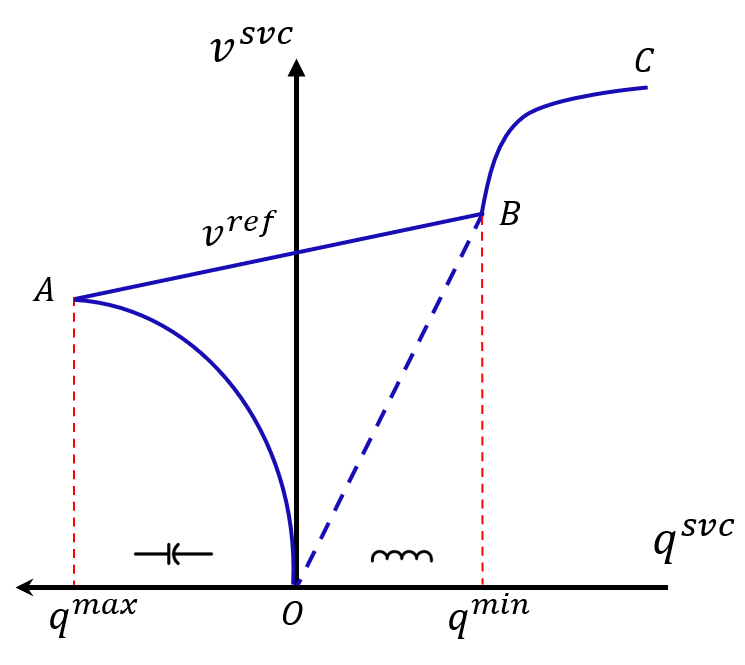
\includegraphics[width=\textwidth]{svc_linear_with_q.png}
		{\footnotesize (a) SVC linear with $Q$.}
	\end{minipage}
	\hfill
	\begin{minipage}{0.48\columnwidth}
		\centering
		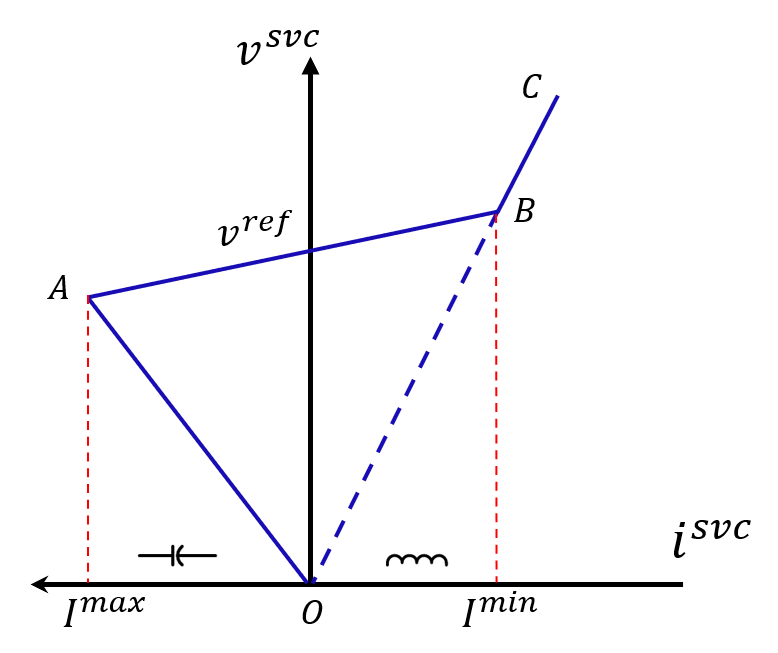
\includegraphics[width=\textwidth]{svc_linear_with_i.png}
		{\footnotesize (b) SVC linear with $I$.}
	\end{minipage}
	\caption{SVC control modes configurations.}
	\label{fig:svc_configurations}
\end{figure}
% ====================================================================================================================================
\vspace{-0.6cm}
\subsection{Line-Commutated Converter (LCC)}
The steady-state modeling of LCC-HVDC systems used in this work follows classical converter relationships, including converter-side voltages, 
current, control angles, and commutation effects \cite{ref13,ref14}. These relationships provide the analytical basis for representing rectifier 
and inverter operation in AC/DC power flow studies as shown in Fig. \ref{fig:lcc_configuration}.
The LCC system is modeled using a unified set of equations for both rectifier ($k=r$) and inverter ($k=i$) terminals \cite{ref15}. For each 
pole $h \in \mathcal{H}$, where $\mathcal{H}$ represents the set of all active DC poles, the DC voltage $V^{dc,h}_k$ is expressed as the ideal 
no-load voltage term plus the commutation reactance drop:
\begin{align}
	\label{eq:vdc_universal}
	V^{dc,h}_k = N^h_k \left(\frac{3 \sqrt{2}}{\pi}\frac{a^h_k V^{ac,h}_k}{T^h_k} \cos{\theta^h_k} + s_k\frac{3 X^{h}_k}{\pi} I^{dc,h}_k\right), \nonumber \\
	\forall h \in \mathcal{H}, \, k \in \{r,i\},
\end{align}
where $s_r=-1$ for the rectifier and $s_i=+1$ for the inverter, which physically accounts for the polarity change and internal voltage drop across 
the bridges under commutation. The parameter $\theta^h_k$ denotes the operational control angle mapped to each terminal mode; 
specifically, $\theta^h_r = \alpha^h_r$ represents the firing delay angle for the rectifier, whereas $\theta^h_i = \gamma^h_i$ represents 
the minimum extinction angle for the inverter. Furthermore, $N^h_k$ is the number of bridges that the converter station possesses for pole $h$ 
at terminal $k$, $a^h_k$ is the transformer ratio, $T^h_k$ is the tap ratio, $X^h_k$ is the commutation reactance, and $I^{dc,h}_k$ is the DC 
current flowing through the link.

The commutation process induces a phase displacement between the AC voltage and fundamental AC current. The corresponding overlap angle $\mu^h_k$ 
and power factor angle $\phi^h_k$ for each pole $h \in \mathcal{H}$ and terminal $k \in \{r,i\}$ are governed by:
\begin{align}
	\label{eq:overlap_angle_fix}
	\mu^h_k  & = \cos^{-1}\left(\cos\theta^h_k-\frac{\sqrt{2}\,I^{dc,h}_k X^{h}_k T^h_k}{a^h_k V^{ac,h}_k}\right)-\theta^h_k, \\
	\label{eq:phi_angle_fix}
	\phi^h_k & = \tan^{-1}\left(
	\frac{\sin(2\theta^h_k+2\mu^h_k)-\sin(2\theta^h_k)+2\mu^h_k}
	{\cos(2\theta^h_k)-\cos(2\theta^h_k+2\mu^h_k)}
	\right).
\end{align}
To guarantee mathematical and physical consistency within the NLP optimization framework, the argument of the inverse cosine in 
\eqref{eq:overlap_angle_fix} is strictly constrained to the domain $[-1, 1]$, preventing non-convergence during high DC current or depressed 
AC voltage states.

The \textit{RMS} AC current $I^{ac,h}_k$ at the converter transformer is proportional to the DC current, while the reactive power 
variable $Q^{ac,h}_k$ at the AC interface is derived for all $h \in \mathcal{H}$ and $k \in \{r,i\}$ as follows:
\begin{align}
	I^{ac,h}_k & = \frac{\sqrt{6}}{\pi}N^h_k I^{dc,h}_k, \label{eq:iac_rms}                        \\
	Q^{ac,h}_k & = \sqrt{3}\, I^{ac,h}_k (a^h_k V^{ac,h}_k / T^h_k)\sin\phi^h_k. \label{eq:hvdc_q}
\end{align}
In the nodal balance, the active power terms $P^{ac,h}_{r}$ and $P^{ac,h}_{i}$ are treated as fixed setpoints specified by the system data models, 
representing a withdrawal at the rectifier bus and an injection at the inverter bus, respectively. Conversely, because line-commutated converters 
inherently consume reactive power regardless of power flow direction, both $Q^{ac,h}_{r}$ and $Q^{ac,h}_{i}$ are modeled strictly as reactive power 
withdrawals. These variables are directly integrated into the nodal power balance equations \eqref{eq:power_flow_1} and \eqref{eq:power_flow_2}. Finally, 
operational feasibility and equipment limits are enforced across all components by:
\begin{align}
	T^{\min,h}_k      & \leq T^h_k \leq T^{\max,h}_k, \quad \forall h \in \mathcal{H}, \, k\in\{r,i\}, \\
	\alpha^{\min,h}_r & \leq \alpha^h_r \leq \alpha^{\max,h}_r, \quad \forall h \in \mathcal{H},       \\
	\gamma^{\min,h}_i & \leq \gamma^h_i \leq \gamma^{\max,h}_i, \quad \forall h \in \mathcal{H}.
\end{align}

\begin{figure*}[!t]
	\centering
	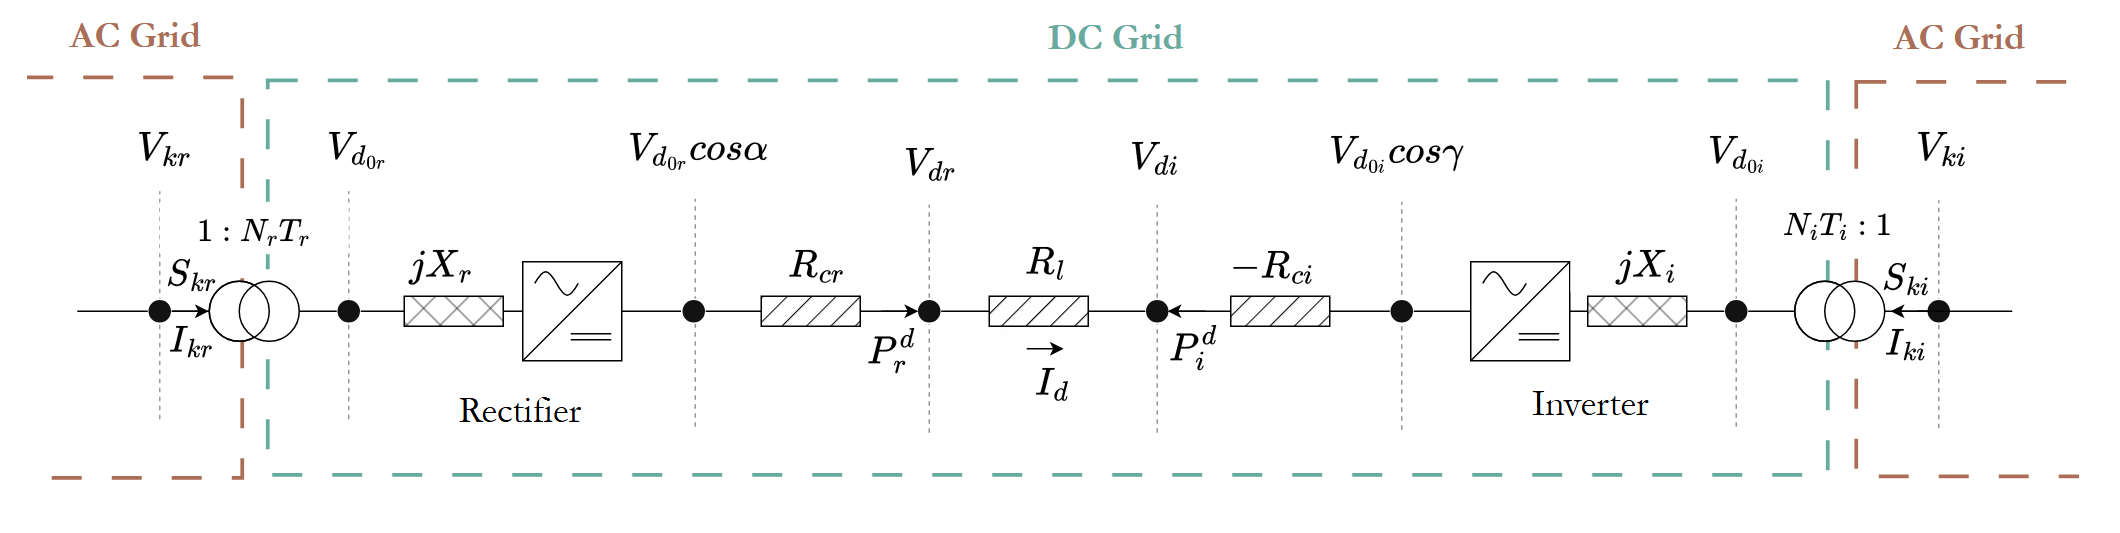
\includegraphics[width=7in]{lcc_converters.png}
	\caption{LCC-HVDC converter stations and circuit representation.}
	\label{fig:lcc_configuration}
\end{figure*}
% ====================================================================================================================================
\section{Simulation Process}

The proposed model is implemented in Python using the Pyomo optimization framework and solved via the Ipopt solver. The simulation starts by 
parsing Anarede files (.pwf) into a readable open-source format (.dat), followed by the execution of the AC/DC power flow model. The post-optimization 
phase involves verifying SVC operational status; if reactive power limits are violated, the algorithm iteratively adjusts setpoints according to the 
control logic defined in \eqref{eq:svc_logic} and solves the system again. This ensures that the final operating point is physically feasible and is 
within the device saturation limits. Validation is then performed by comparing the proposed model results against Anarede. Numerical differences are 
expected, since the software uses Newton Raphson based algorithms. These differences are particularly evident near operational boundaries, such as 
converter transformer tap limits or maximum firing angles ($\alpha_{max}, \gamma_{max}$), where the two solvers may converge on different but equally 
feasible points.

\begin{algorithm}[!t]
\caption{Residual-based optimization AC/DC power flow}
\label{alg:residual_power_flow}
\begin{algorithmic}[1]
\STATE Parse and validate the network, schedules, controls, and tolerances.
\STATE Reduce eligible near-zero-impedance branches and build effective connectivity.
\STATE Initialize voltages, angles, controls, and signed residuals from the input state.
\STATE Fix scheduled active generation unless redispatch was explicitly requested.
\STATE Build AC, FACTS, LCC, control, per-bus residual, and aggregate residual constraints.
\STATE Minimize \eqref{eq:obj_function} with Ipopt.
\STATE Accept convergence only if termination is accepted and all local and aggregate residual tests pass.
\STATE Report voltage and branch-limit violations separately from convergence.
\STATE Update saturated SVC control regions and repeat when a control-state change is required.
\end{algorithmic}
\end{algorithm}

% =================================================================================================================================================================
\begin{figure}[!ht]   % <--- Changed from [H] to [!ht]
	\centering
	\includegraphics[width=\columnwidth]{brazil_sys.png}
	\caption{BIPS transmission network.}
	\label{fig:bips_transmission_network}
\end{figure}
% \begin{figure}[!htbp]
% \centering
% \includegraphics[width=2.0in]{img/brazil_sys.png}
% \caption{BIPS transmission network.}
% \label{fig:bips_transmission_network}
% \end{figure}
% \FloatBarrier   

\section{Numerical Results}

\subsection{BIPS Data Model}

The data model used to represent the BIPS transmission network, as seen in Figure \ref{fig:bips_transmission_network}, consists of 7308 buses, 
6477 lines, 3861 two-winding transformers, 68 CSCs, 44 SVCs, 321 line shunts, 1961 bus/line capacitor/reactor banks, 1299 generators and 
2736 loads. The operating snapshots are based on cases released by the Brazilian Independent System Operator \cite{ref16}.

\begin{table}[htb]
	\centering
	\footnotesize
	\caption{LCC line parameters in the BIPS.}
	\label{tab:summary_lcc_links}
	\renewcommand{\arraystretch}{1.2}
	\setlength{\tabcolsep}{6pt}
	\begin{tabular}{ccccc}
		\hline
		\textbf{\begin{tabular}[c]{@{}c@{}}Line\\ Name\end{tabular}}    &
		\textbf{\begin{tabular}[c]{@{}c@{}}Voltage\\ (kV)\end{tabular}} &
		\textbf{\begin{tabular}[c]{@{}c@{}}Power\\ (MW)\end{tabular}}   &
		\textbf{\begin{tabular}[c]{@{}c@{}}Pole\\ No.\end{tabular}}     &
		\textbf{$\alpha / \gamma$ ($^\circ$)}                                                                 \\ \hline
		Itaipu                                                          & 600/587.7 & 1050/1018 & 4 & 15/17   \\ \hline
		Madeira 1                                                       & 600/557.2 & 1500/1393 & 2 & 15/17   \\
		Madeira 2                                                       & 600/560.4 & 1500/1401 & 2 & 13/18   \\ \hline
		Belo Monte 1                                                    & 800/765.2 & 2000/1913 & 2 & 14.3/15 \\
		Belo Monte 2                                                    & 800/759.5 & 2000/1899 & 2 & 18.4/17 \\ \hline
	\end{tabular}
\end{table}

As part of this study, the main LCC-HVDC corridors currently relevant to BIPS operation are explicitly modeled. These include the Itaipu 
link (Foz do Igua\c{c}u--Ibi\'una), the Madeira complex (Santo Ant\^onio--Araraquara, ABB and Areva bipoles), and the Belo Monte transmission 
link (Xingu--Estreito and Xingu--Terminal Rio). In total, the implemented set comprises 12 poles organized as three major LCC schemes: four poles 
at 600~kV for Foz/Ibi\'una, four poles at 600~kV for Santo Ant\^onio/Araraquara, and four poles at 800~kV for the Xingu corridors, with nominal pole 
powers in the range of approximately 1566--2000~MW. Their representative operating settings are summarized in Table~\ref{tab:summary_lcc_links}.

\subsection{Model Validation}
To validate the proposed AC/DC power flow model, the corresponding analysis is performed on the equivalent BIPS model focusing on the point-to-point 
DC configuration on the LCC-HVDC links described on Table \ref{tab:summary_lcc_links}. Using a flat start configuration on the AC side, and keeping 
DC voltage constant on one of each converter stations, the results for the equivalent BIPS are shown in Fig.~\ref{fig:equivalent_bips_model_ac_components} 
and Fig.~\ref{fig:equivalent_bips_model_dc_components}, respectively.

It can be observed that the proposed AC/DC power flow model tracks the AC voltage magnitudes, phase angles, generator active and reactive power outputs, 
branch flows, and the control setpoints of the FACTS and LCC-HVDC devices across the equivalent and full BIPS network. To quantify the similarity between 
the proposed AC/DC model and Anarede, an $R^2$ coefficient of determination was applied across the validation datasets, confirming a high fit on the results.

% ====================================================================================
% UNIFIED FIGURE 1: AC COMPONENTS VALIDATION
% Placed early to anchor the initial description of the equivalent system results.
% ====================================================================================
\begin{figure}[!htbp]
	\centering
	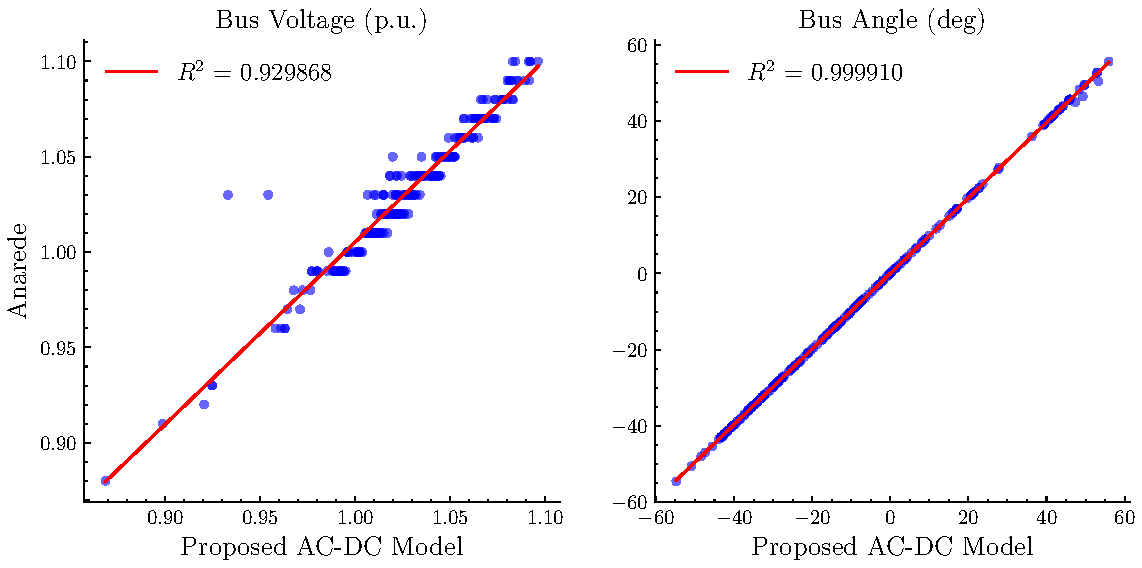
\includegraphics[width=0.95\columnwidth]{LENA_CASO_FINAL_EQV2020_DC_Full_bus_voltage_angle_results.pdf} \\[0.3em]
	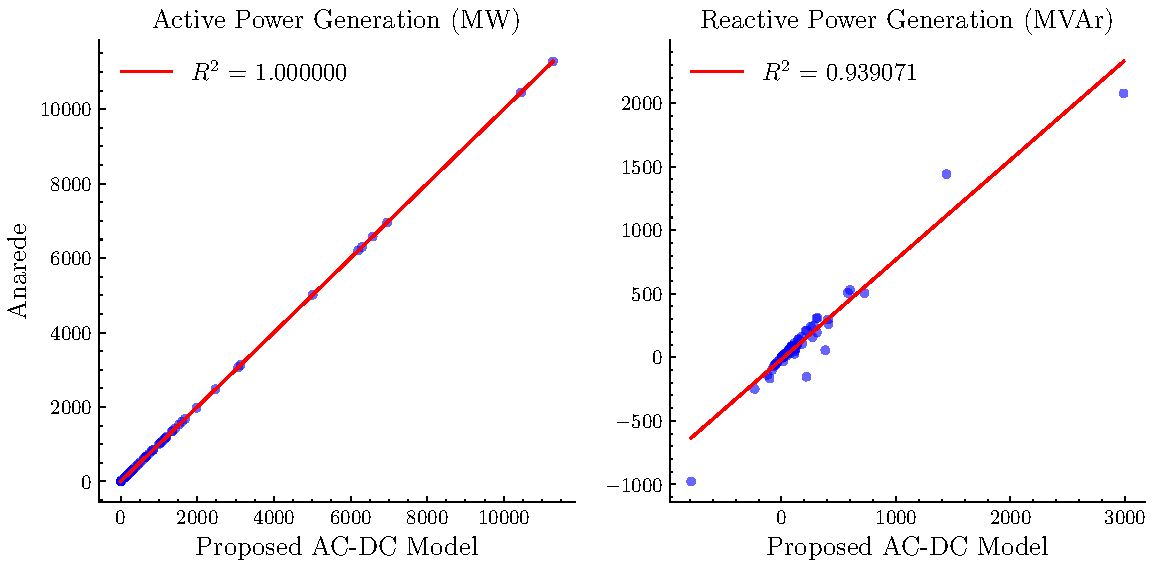
\includegraphics[width=0.95\columnwidth]{LENA_CASO_FINAL_EQV2020_DC_Full_generation_active_reactive.pdf} \\[0.3em]
	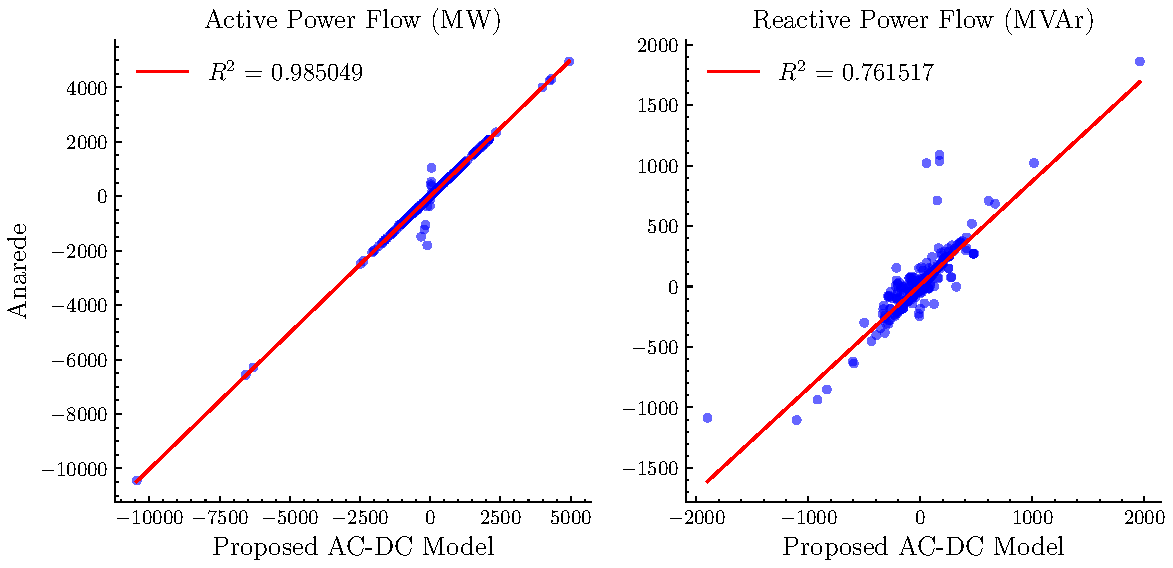
\includegraphics[width=0.95\columnwidth]{LENA_CASO_FINAL_EQV2020_DC_Full_branch_flow_active_reactive.pdf} \\[0.3em]
	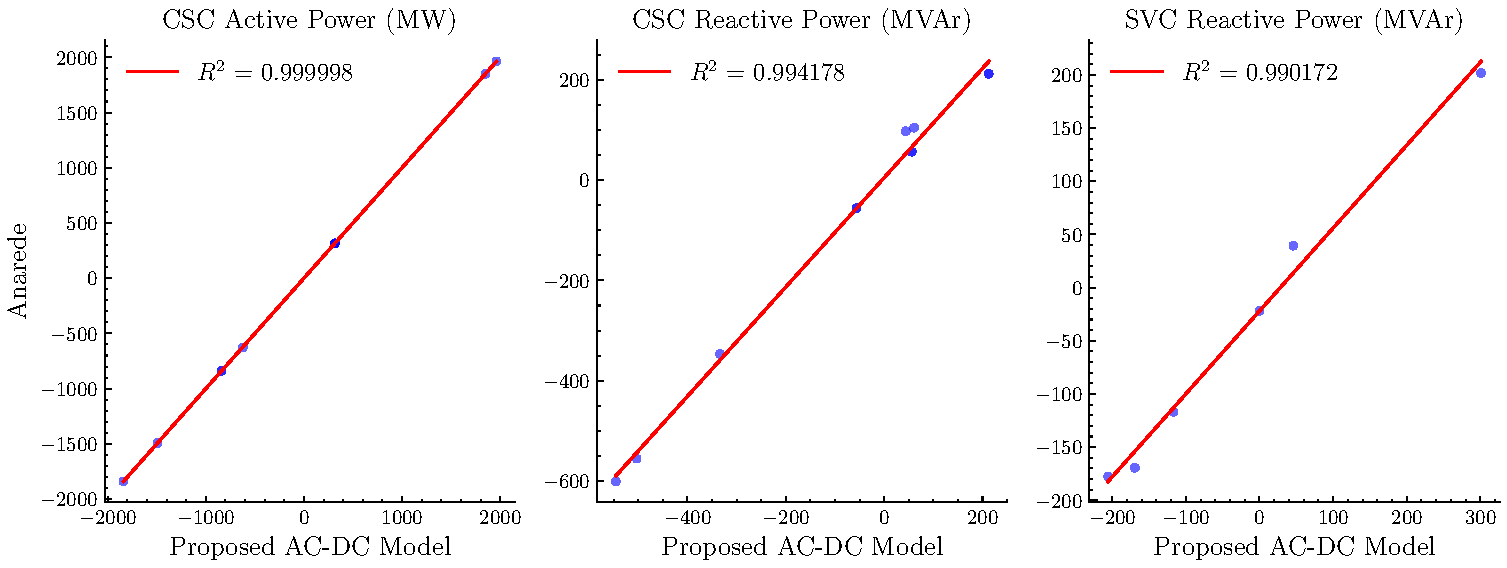
\includegraphics[width=0.95\columnwidth]{LENA_CASO_FINAL_EQV2020_DC_Full_csc_svc_results.pdf}
	\caption{Validation of equivalent BIPS model at AC components.}
	\label{fig:equivalent_bips_model_ac_components}
\end{figure}

The mismatches observed when comparing the results with Anarede are primarily driven by differences in core modeling approaches and power flow 
assumptions. Because a NLP problem of this scale possesses multiple local solutions, the solver successfully converges to a physically feasible 
operating point around the feasible set.

Furthermore, minor variations in the converter firing ($\alpha$) and extinction ($\gamma$) angles are expected. While the acceptable operational 
limits for these angles typically span from 5° to 90°, in steady-state operation it is preferred to have small angle values for safe operation and 
to avoid commutation failure as shown in Table \ref{tab:summary_lcc_links}; in this simulation, the control angles variation was in a range from 15° 
to 23°. Because these parameters are handled within an optimization framework, the solver's primary objective is to ensure they converge within 
coherent operational boundaries rather than matching the exact value. Specifically, the NLP formulation evaluates these variables from a system-wide 
perspective, balancing active and reactive power constraints across the entire network and optimizing the control angles to achieve a feasible solution.

% ====================================================================================
% UNIFIED FIGURE 4: EQUIVALENT DC COMPONENTS
% Inserted right after discussing the converter angles optimization.
% ====================================================================================
\begin{figure}[!htbp]
	\centering
	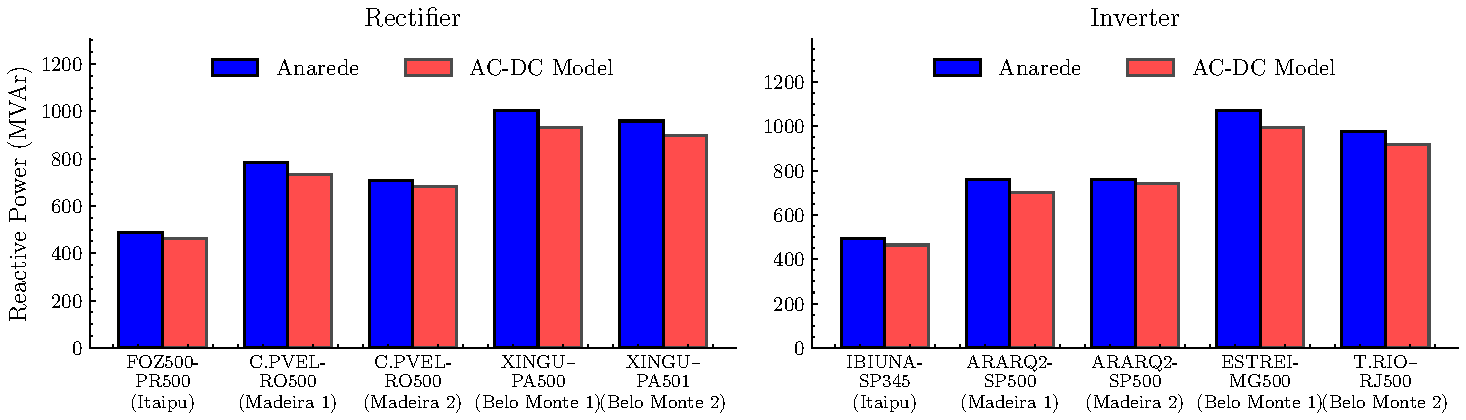
\includegraphics[width=0.95\columnwidth]{LENA_CASO_FINAL_EQV2020_DC_Full_hvdc_reactive_power.pdf} \\[0.5em]
	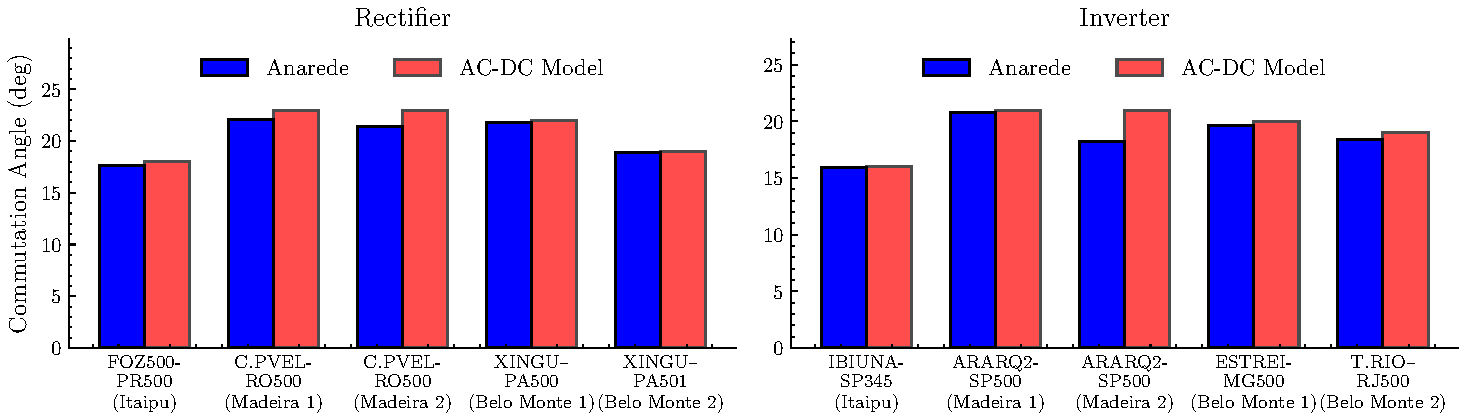
\includegraphics[width=0.95\columnwidth]{LENA_CASO_FINAL_EQV2020_DC_Full_hvdc_commutation_angle.pdf} \\[0.5em]
	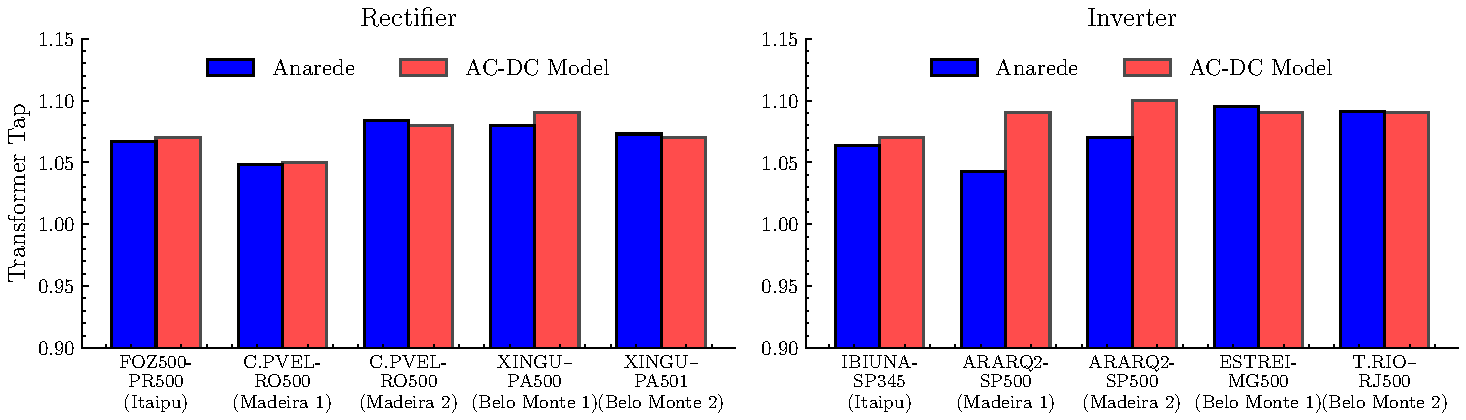
\includegraphics[width=0.95\columnwidth]{LENA_CASO_FINAL_EQV2020_DC_Full_hvdc_transformer_tap.pdf}
	\caption{Validation of equivalent BIPS model at DC components.}
	\label{fig:equivalent_bips_model_dc_components}
\end{figure}

Unlike the active power results, reactive power are highly sensitive to small network modeling variations. In the proposed formulation, the 
transformer model is simplified by applying a tap ratio configuration directly to the power flow equations. The bus and line shunts are directly 
added into the bus susceptance ($B$) values. These simplified representations can modify the localized reactive power distribution across the 
network. Consequently, mismatches can be observed when comparing the results with a commercial software like Anarede.

To evaluate the performance and scalability of the proposed AC/DC power flow model, the 7308-bus BIPS model was simulated under a normal steady-state 
operation mode for the LCC-HVDC. The resulting power flow profiles demonstrate that the active and reactive generator outputs, AC bus voltage magnitudes 
and phase angles, FACTS and LCC-HVDC terminal parameters are kept within their operational boundaries. These profiles are observed 
in Fig.~\ref{fig:bus_validation} and Fig.~\ref{fig:branch_validation}.

% ====================================================================================
% UNIFIED FIGURE 2: BUS & GEN VALIDATION
% Placed directly under the scalability paragraph where it is referenced.
% ====================================================================================
\begin{figure}[!htbp]
	\centering
	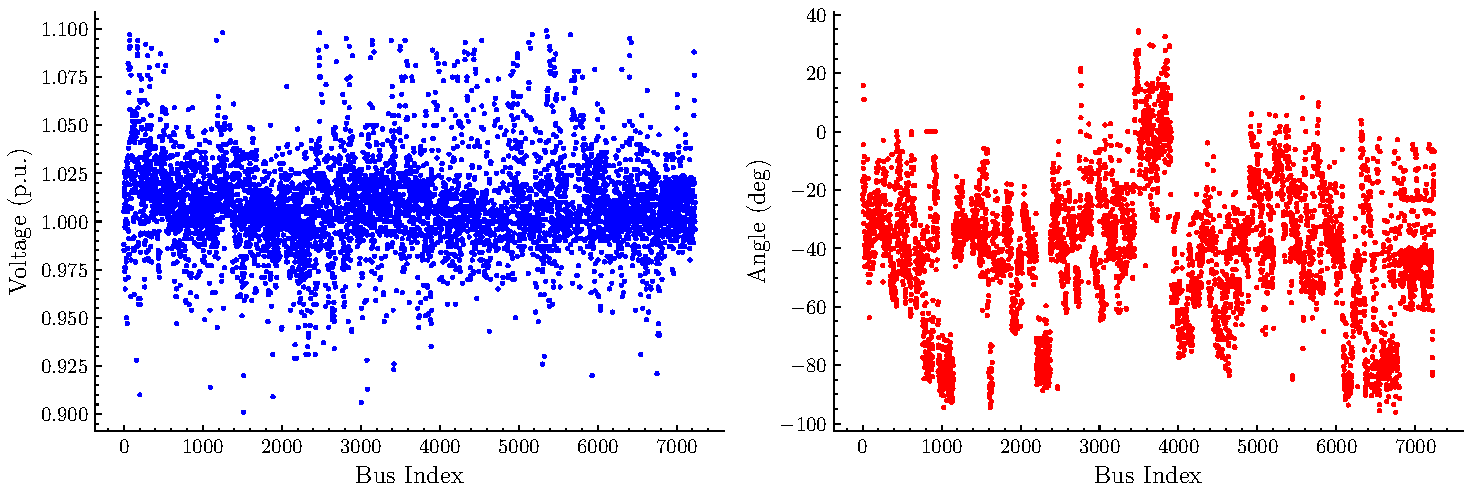
\includegraphics[width=0.95\columnwidth]{LEN_A_4_2020_SECO_2023VM_SE_EXP_N_4DC_bus_voltage_angle.pdf} \\[0.5em]
	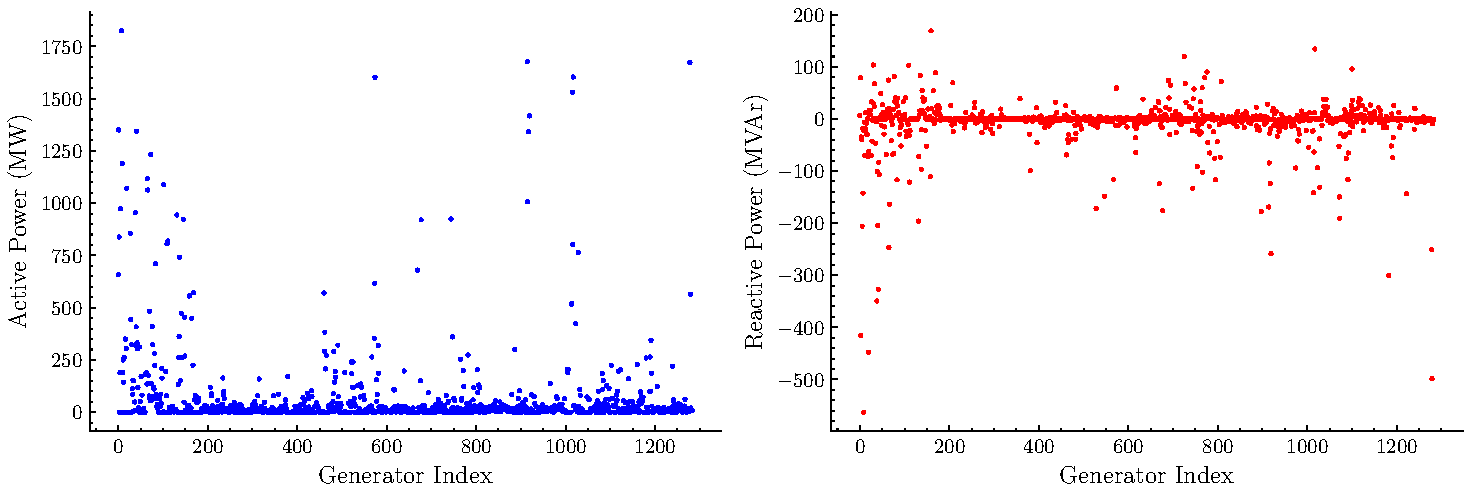
\includegraphics[width=0.95\columnwidth]{LEN_A_4_2020_SECO_2023VM_SE_EXP_N_4DC_generation_scatter.pdf}
	\caption{AC/DC power flow results for buses and generators.}
	\label{fig:bus_validation}
\end{figure}
To support the heavy transmission conditions of high active power flows transmitted over the long-distance LCC-HVDC systems, the 
converter transformer tap positions are controlled within an physical range of $0.9$ to $1.2$. Keeping the tap ratios in this range 
is important in normal operating mode, as they adjust the AC side voltage to minimize the converter firing angles ($\alpha$) and extinction 
angles ($\gamma$), directly minimizing the high reactive power demand consumed by the converter stations, as can be seen in 
Fig.~\ref{fig:bips_model_ac_components}.
% ====================================================================================
% UNIFIED FIGURE 3: BRANCH & SVC VALIDATION
% Placed here alongside the final discussions of FACTS devices and computational cost.
% ====================================================================================
\begin{figure}[!htbp]
	\centering
	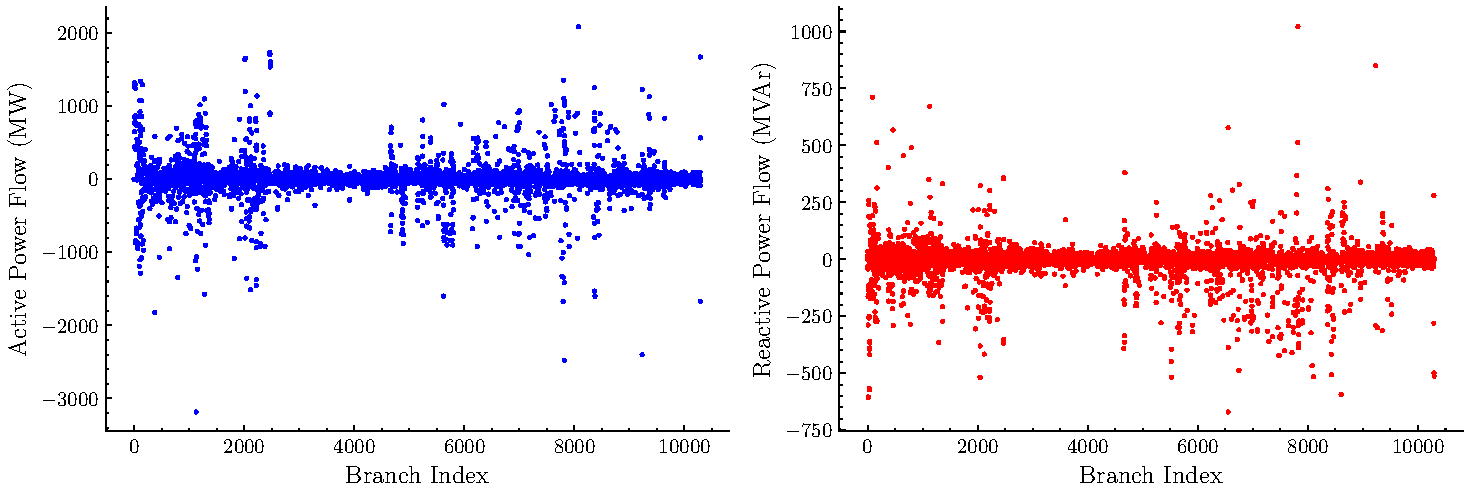
\includegraphics[width=0.95\columnwidth]{LEN_A_4_2020_SECO_2023VM_SE_EXP_N_4DC_branch_flow_scatter.pdf} \\[0.5em]
	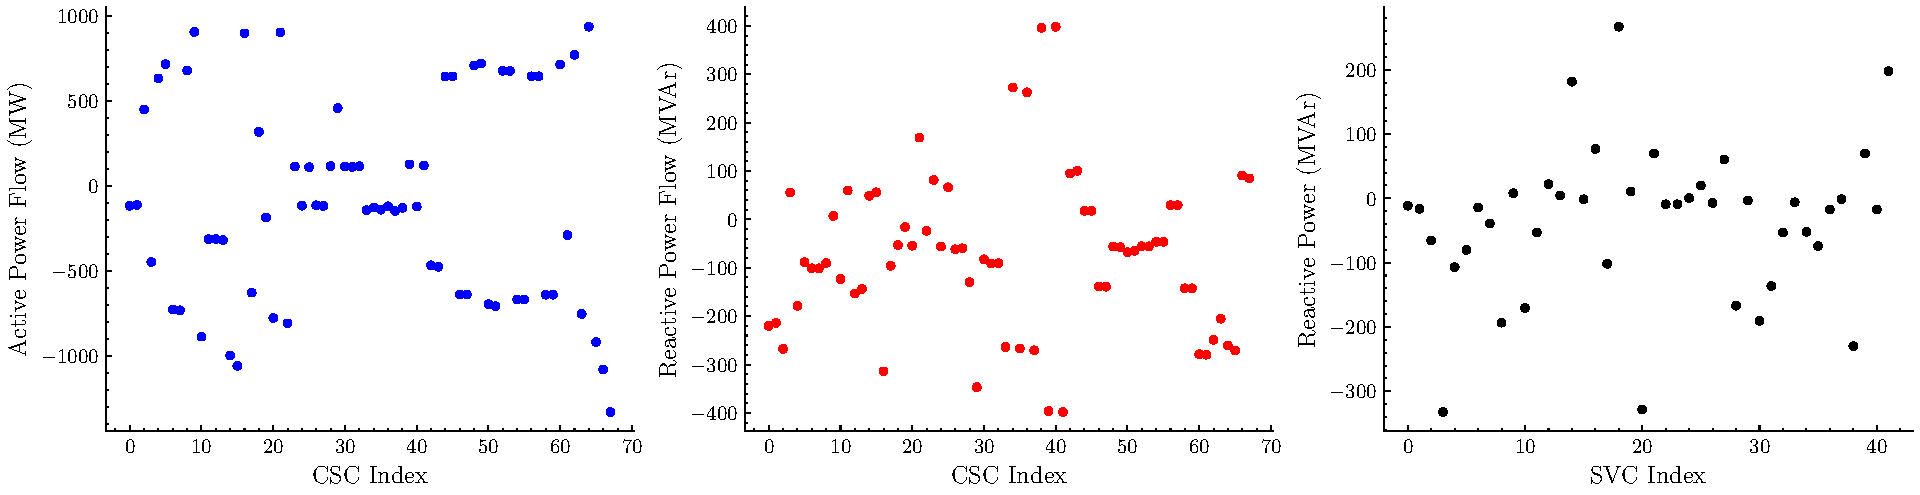
\includegraphics[width=0.95\columnwidth]{LEN_A_4_2020_SECO_2023VM_SE_EXP_N_4DC_dcsc_dcer_scatter.pdf}
	\caption{AC/DC power flow results for branches and FACTS devices.}
	\label{fig:branch_validation}
\end{figure}
Additionally, the highly meshed nature of the BIPS requires active and reactive flow control via FACTS devices, without them the system would 
not converge to a feasible point. The proposed model incorporates these formulations into the nodal power balance equations. The active and 
reactive power through the CSC is controlled by active ($P_{csc}$) and reactive ($Q_{csc}$) flow constraints, which adjust them based on the 
equivalent series reactance ($X_{esp}$). Voltage support and reactive power control are enforced at SVC buses. The model implements piecewise 
voltage control constraints that govern the reactive power injection ($Q_c$) based on localized voltage deviations ($V - V_0$) and slope 
characteristics ($I_{ncl}$), accounting for physical operating limits ($Q_{cn}, Q_{cm}$).
% ====================================================================================
% UNIFIED FIGURE 4: FULL BIPS DC COMPONENTS
% Staggered here to visually support the transformer tap ratio and angle analysis.
% ====================================================================================
\begin{figure}[!htbp]
	\centering
	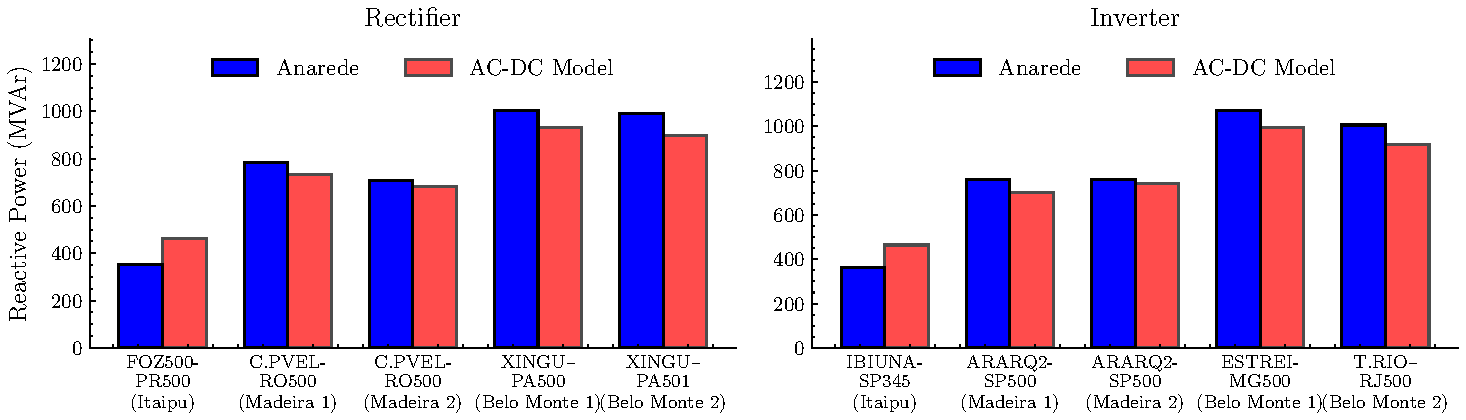
\includegraphics[width=0.95\columnwidth]{LEN_A_4_2020_SECO_2023VM_SE_EXP_N_DC_Full_hvdc_reactive_power.pdf} \\[0.5em]
	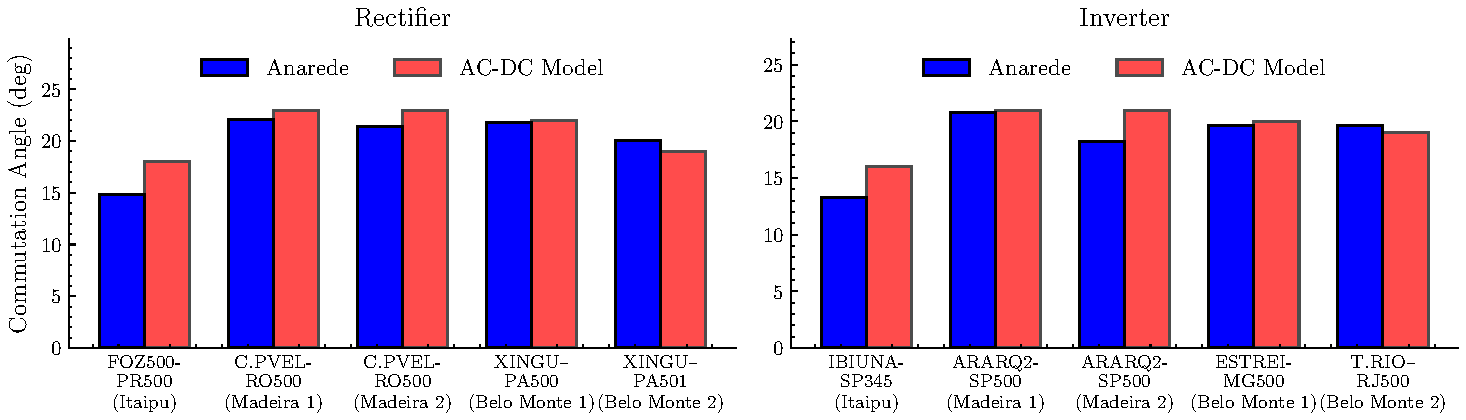
\includegraphics[width=0.95\columnwidth]{LEN_A_4_2020_SECO_2023VM_SE_EXP_N_DC_Full_hvdc_commutation_angle.pdf} \\[0.5em]
	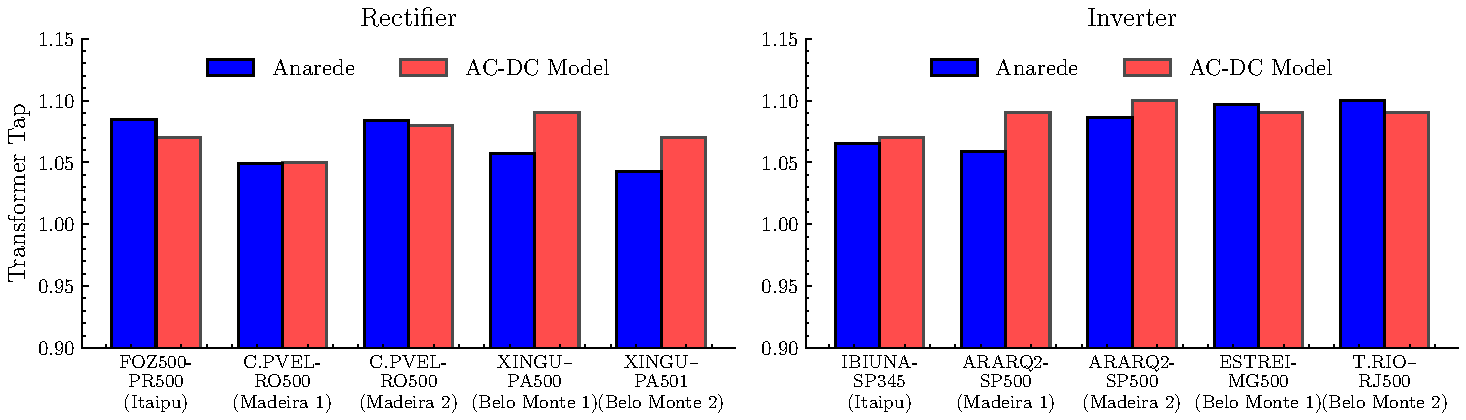
\includegraphics[width=0.95\columnwidth]{LEN_A_4_2020_SECO_2023VM_SE_EXP_N_DC_Full_hvdc_transformer_tap.pdf}
	\caption{Validation of BIPS model at DC components.}
	\label{fig:bips_model_ac_components}
\end{figure}
\subsection{Computational Scalability}

Table~\ref{tab:scalability} reports fresh-process timings on Windows 11 with Python 3.13.3, Pyomo 6.10.1, and Ipopt 3.14.19. All six cases
met the termination and balance-residual criteria. The three 11,250-bus snapshots required 55--59 iterations and 21.3--23.2~s total time,
showing consistent behavior across operating snapshots. The optimization model is nevertheless slower than a dedicated sparse Newton solve,
as quantified below, because it handles residuals, controls, and operational slacks in one NLP.

\begin{table*}[!t]
\centering
\footnotesize
\caption{NLP scalability results from saved benchmark runs.}
\label{tab:scalability}
\setlength{\tabcolsep}{5pt}
\begin{tabular}{lrrrrrrrr}
\hline
\textbf{Case} & \textbf{Buses} & \textbf{Branches} & \textbf{Variables} & \textbf{Constraints} & \textbf{Iter.} & \textbf{Build (s)} & \textbf{Solve (s)} & \textbf{Total (s)} \\ \hline
EQV-2020   & 236    & 583    & 2,963   & 1,758  & 21 & 0.04 & 0.23 & 0.32 \\
BIPS-2020  & 6,871  & 9,463  & 83,430  & 53,641 & 42 & 1.63 & 8.42 & 11.63 \\
ONS-2020   & 6,871  & 9,463  & 83,430  & 53,641 & 42 & 1.25 & 8.66 & 11.80 \\
BIPS-00:00 & 11,250 & 14,478 & 133,237 & 87,102 & 55 & 1.94 & 16.75 & 21.29 \\
BIPS-02:00 & 11,250 & 14,478 & 133,252 & 87,102 & 57 & 2.40 & 18.13 & 23.15 \\
BIPS-02:30 & 11,250 & 14,478 & 133,213 & 87,100 & 59 & 2.34 & 18.30 & 23.18 \\ \hline
\end{tabular}
\end{table*}

\subsection{Stressed-Condition Robustness}

The robustness experiment applied active-load multipliers, a reactive-load multiplier, a 50\% reduction of finite generator reactive
ranges, and deterministic removal of one in-service branch. Table~\ref{tab:stress_results} uses B for a balance-converged point with one or
more reported voltage or branch-limit violations and F for failure of the accepted-termination or residual test. Thus, B is not a claim of
operational security. The 11,250-bus snapshot remained balanced in every tested perturbation, whereas the equivalent and medium cases exposed
clear loadability and contingency limits. This behavior demonstrates robustness on the tested full snapshot, not universal convergence.

\begin{table}[!t]
\centering
\footnotesize
\caption{NLP outcome under stressed conditions.}
\label{tab:stress_results}
\setlength{\tabcolsep}{3.5pt}
\begin{tabular}{lcccccc}
\hline
\textbf{Case} & \textbf{Base} & \textbf{$P_{1.1}$} & \textbf{$P_{1.2}$} & \textbf{$Q_{1.2}$} & \textbf{$Q_{lim,0.5}$} & \textbf{N--1} \\ \hline
BIPS-00:00 & B & B & B & B & B & B \\
EQV-2020   & B & F & F & B & B & B \\
BIPS-2020  & B & F & F & B & B & F \\ \hline
\multicolumn{7}{l}{\scriptsize B: balance-converged with operational violations; F: failed convergence test.}
\end{tabular}
\end{table}

\subsection{Direct Method Comparison}

For a controlled comparison, the NLP, Newton executable, and fast-decoupled entry point were run on three cases at load factors 1.0, 1.1,
and 1.2. As shown in Table~\ref{tab:method_comparison}, all methods solved the three normal points. The NLP additionally solved the two
stressed 11,250-bus points, giving five accepted points out of nine. Its median solution time was correspondingly higher. The fast-decoupled
entry produced the same results as Newton because cases containing LCC devices are routed internally to the coupled Newton solver; its row
must therefore not be interpreted as an independent fast-decoupled result.

\begin{table}[!t]
\centering
\footnotesize
\caption{Direct convergence comparison over nine scenarios.}
\label{tab:method_comparison}
\setlength{\tabcolsep}{5pt}
\begin{tabular}{lcccr}
\hline
\textbf{Method} & \textbf{Normal} & \textbf{Stressed} & \textbf{Success} & \textbf{Median (s)} \\ \hline
NLP              & 3/3 & 2/6 & 55.56\% & 16.400 \\
Newton           & 3/3 & 0/6 & 33.33\% & 3.287 \\
Fast entry$^{a}$ & 3/3 & 0/6 & 33.33\% & 3.267 \\ \hline
\multicolumn{5}{l}{\scriptsize $^{a}$LCC cases routed to the coupled Newton implementation.}
\end{tabular}
\end{table}

% ===========================================================================================
\section{Conclusions}

This paper presents an open-source optimization-based integrated AC/DC power flow model for large systems with LCC-HVDC and FACTS devices.
The residual-based NLP simultaneously represents nonlinear AC equations, DC constraints, converter controls, and bounded feasibility measures.
Validation against Anarede shows consistent operating points under the stated modeling assumptions. All six scalability cases converged, including
three 11,250-bus snapshots, and the NLP solved two stressed scenarios that the compared Newton-based entries did not. These results support the
tractability and improved robustness of the formulation for the tested cases, but also show that convergence and operational acceptability are
different outcomes: every solved comparison point retained at least one reported voltage or branch-limit violation. Future work should enforce or
repair these limits through control switching and continuation strategies and should broaden comparisons using a native fast-decoupled method on
compatible AC-only cases.

% ==============================================================================================================
\begingroup
\hbadness=10000
\begin{thebibliography}{1}
	\bibliographystyle{IEEEtran}


	\bibitem{ref1}
	B. Stott, "Review of load-flow calculation methods". In Proceedings of the IEEE, vol. 62, no. 7, pp. 916-929, July 1974, doi: 10.1109/PROC.1974.9544.

	\bibitem{ref2}
	E. H. Watanabe, P. G. Barbosa, K. C. Almeida, and G. N. Taranto, "Tecnologia FACTS - Tutorial". \textit{SBA Controle \& Automação}, vol. 9, no. 1, pp. 1--15, 1998.

	\bibitem{ref3}
	J. Beerten, S. Cole, and R. Belmans, “Generalized steady-state VSC MTDC model for sequential AC/DC power flow algorithms,” IEEE Trans. Power Syst., vol. 27, no. 2, pp. 821–829, May.
	2012.

	\bibitem{ref4}
	J. Beerten and R. Belmans, "Development of an open source power flow software for high voltage direct current grids and hybrid ac/dc systems: MatACDC". IET Gener. Transm. Distrib., vol. 9, no. 10, pp. 966–974, 2015.

	\bibitem{ref5}
	J. Lei, T. An, Z. Du, and Z. Yuan. "A general unified ac/dc power flow algorithm with MTDC". IEEE Trans. on Power Syst., vol. 32, no. 4, pp. 2837–2846, 2016.

	\bibitem{ref6}
	E. Acha, C. R. Fuerte-Esquivel, H. Ambriz-P\'erez, and C. Angeles-Camacho, "FACTS: Modeling and Simulation in Power Networks". Chichester, U.K.: John Wiley \& Sons, 2004, doi: 10.1002/0470020164.

	\bibitem{ref7}
	W. A. Bukhsh, "On Solving the Load Flow Problem as an Optimization Problem". Univ. Strathclyde, Glasgow, U.K., Tech. Rep., 2018. [Online]. Available: https://pure.strath.ac.uk

	\bibitem{ref8}
	A. Wächter and L. T. Biegler, "On the Implementation of a Primal-Dual Interior Point Filter Line Search Algorithm for Large-Scale Nonlinear Programming". \textit{Math. Program.}, vol. 106, no. 1, pp. 25--57, 2006.

	\bibitem{ref9}
	CEPEL, DRE, "Network Analysis Program (ANAREDE), Version 10.01.00: User Manual", Centro de Pesquisas de Energia El\'etrica, Rio de Janeiro, Brazil, Sep. 2015. [Online]. Available: http://www.cepel.br

	\bibitem{ref10}
	L. Braz, C. Castro, and C. Murati, "A critical evaluation of step size optimization based load flow methods", IEEE Transactions on Power Systems, vol. 15, no. 1, pp. 202–207, 2000.

	\bibitem{ref11}
	C. K. Jat, F. G. Puricelli, J. Beerten, H. Ergun and D. Van Hertem, "Unified Power Flow Model for Bipolar HVDC Grids in Unbalanced Operation", in IEEE Transactions on Power Systems, vol. 41, no. 3, pp. 2005-2017, May 2026, doi: 10.1109/TPWRS.2025.3641544.

	\bibitem{ref12}
	Padiyar, K.R, "FACTS Controllers in Power Transmission and Distribution". New Age International Pvt. Limited, New Delhi. 2027.

	\bibitem{ref13}
	J. Arrillaga, "High Voltage Direct Current Transmission", 2nd ed. London, U.K.: The Institution of Engineering and Technology, 2008.

	\bibitem{ref14}
	J. Arrillaga and B. Smith, "AC-DC Power System Analysis". London, U.K.: The Institution of Electrical Engineers, 1998.

	\bibitem{ref15}
	PTI, Inc., "PSS\textsuperscript{\textregistered}E 34.9.5 Program Application Guide, Volume 1". Schenectady, NY, USA: Siemens Power Technologies International, May 2022.

	\bibitem{ref16}
	Operador Nacional do Sistema Elétrico (ONS), "ONS (Operador Nacional do Sistema Elétrico)", 2025. [Online]. Available: https://www.ons.org.br/. Accessed: Apr. 20, 2025.

\end{thebibliography}
\endgroup

\end{document}


